\documentclass{article}

\usepackage[utf8]{inputenc}
\usepackage[pdftex]{graphicx}
\usepackage[left=3cm,right=3cm,top=3cm,bottom=3cm]{geometry}
\usepackage[T1]{fontenc}
\usepackage[francais,english]{babel}
\frenchbsetup{StandardLists=true}
\selectlanguage{english}


\usepackage{amsmath}
\usepackage{amssymb}
\usepackage{mathtools}
\usepackage{slashbox}


\usepackage{caption}
\usepackage[hidelinks]{hyperref}
\usepackage{xcolor}

\usepackage{listings}

\usepackage{graphicx}

\renewcommand\thesection{\arabic{section}}

\usepackage{fancyhdr}
\pagestyle{fancy}
\fancyhf{}
\fancyhead[R]{\thepage}


\title{[INFO-F409] Learning Dynamics \\ First assignment}
\author{\bsc{BUI QUANG PHUONG} Quang Linh \\ Université libre de Bruxelles - ULB ID : 000427796  \\ MA1 Computer Sciences}
\date{November 2018}

\begin{document}

\maketitle

\tableofcontents

\newpage
\section{The Hawk-Dove game}

\subsection*{Conventions and notations}
First of all, the Hawk-Dove game is modeled by the matrix presented in the \autoref{table:payoffMatrix}. 

\begin{center}
\begin{tabular}{|l|r|r|}
  \hline
  			   & Hawk & Dove \\
  \hline
  		   & \hspace{1cm} $\frac{V-D}{2}$ & 0 \\
  	Hawk &	\multicolumn{1}{|l|}{$\frac{V-D}{2}$}		& 	\multicolumn{1}{|l|}{$V$ }		\\
  \hline
    		   & \multicolumn{1}{|r|}{$V$} & \hspace{1cm} $\frac{V}{2}-T$  \\
  Dove &	\multicolumn{1}{|l|}{0}		& 	\multicolumn{1}{|l|}{$\frac{V}{2}-T$}		\\
  \hline
\end{tabular}
\captionof{table}{Payoff matrix of the Hawk-Dove game}
\label{table:payoffMatrix}
\end{center}

The different actions of a player $i \in \{1,2\}$ are denoted by the set $\mathcal{A} = \{H,D\}$ where $H$ is the hawk action and  
$D$ the dove action. Moreover, to denote the different actions payoff, we need an utility function of those actions. This utility function is then written  : 
$$ u_{i}(a_{i}, a_{-i}) $$ such that $a_{i}$ is an action of player $i$ and $a_{-i}$ is the action of the other player where player $i$ choses $a_{i}$. For instance,  $ u_{1}(Hawk, Dove) = V $ and $ u_{2}(Hawk, Dove) = 0 $). \\

In the case of mixed strategies, the notion of \textbf{expected value} of a payoff function is used and is written in the general case :
$$ U_{i}(p_{1}, ... , p_{k }) = p_{k} u(a_{k})$$ where $i$ is a player, $p_{k}$ is the probability that the other player chose the action $a_{k}$. 
In the case of the Hawk-Dove game, the expected value formula would be written such that $k=2$ because it exists only 2 actions, i.e. :  $$ U_{i}(p_{1}, p_{2}) = p_{1} u(a_{1}) + p_{2} u(a_{2})$$

Furthermore, to find Nash equilibria, best responses have to be found. Those one will be highlighted in \colorbox{pink}{red} for the line player considered as player one and \colorbox{green}{green} for the column player considered as player two. 

\subsection{Question 1 - Nash equilibrium}

\subsubsection*{Statement} 
\noindent
\textit{ Find all the (mixed strategy) Nash equilibria of this game. How do the results change when the order of the parameters V, D and T is changed (V>D, D>T, etc.)?}

\subsubsection*{Sign of V, D and T} 
Before starting the analysis, we should remind that $V$ and $D$ are representing respectively the fitness value of winning resources in fight and costs of injury thereby it would not make sense having negative values. $V$ and $D$ are then always positive values. Same for $T$ which is the cost of wasting time. The time wasted is obviously always a positive value. To summarize, 
$$ V, D, T \ge 0 $$  


\subsubsection{First case : $V>D$} 

In the first case, we consider that $V>D$. Therefore, we know that the value of $u_{i}(Hawk, Hawk) = \frac{V-D}{2}$ will be strictly positive. In this case, the choice of both players are quiet easy. As illustrated in \autoref{table:NE-case1}, the Nash equilibrium is $(Hawk, Hawk) \in \mathcal{A}$. Indeed, both players are chosing $Hawk$ because if one of them is switching to $Dove$ then $u_{i}(Hawk,Hawk)$ which was a positive value becomes $u_{1}(Dove,Hawk)$ for player 1 or $u_{2}(Hawk,Dove)$ for player 2 which equals zero. Thus, they obviously prefer to pick $(Hawk,Hawk)$. \\

\begin{center}
\fbox{Nash equilibrium when $(V>D) = \{(Hawk, Hawk)\}$}
\end{center} 

\begin{center}
\begin{tabular}{|l|r|r|}
  \hline
  			   & Hawk & Dove \\
  \hline
  		   & \hspace{1cm} \colorbox{green}{$\frac{V-D}{2}>0$} & 0 \\
  	Hawk &	\multicolumn{1}{|l|}{\colorbox{pink}{$\frac{V-D}{2}>0$}}		& 	\multicolumn{1}{|l|}{\colorbox{pink}{$V$}}		\\
  \hline
    		   & \multicolumn{1}{|r|}{\colorbox{green}{$V$}} & \hspace{1cm} $\frac{V}{2}-T$  \\
  Dove &	\multicolumn{1}{|l|}{0}		& 	\multicolumn{1}{|l|}{$\frac{V}{2}-T$}		\\
  \hline
\end{tabular}
\captionof{table}{Nash equilibrium/Best responses in case 1}
\label{table:NE-case1}
\end{center}

\subsubsection{Second case : $V=D$}
The second case considers the same value for $V$ and $D$ which means that $\frac{V-D}{2} = 0$. The \autoref{table:NE-case2} shows the Nash equilibria for that case. We can see that there doesn't exist only one Nash equilibrium, but three. $(Hawk,Hawk)$ stays a Nash equilibrium in this case, but $(Dove,Hawk)$ and $(Hawk,Dove)$ are now also Nash equilibria. In other words, if player 2 is chosing $Hawk$, the best response to it is whether $(Hawk,Hawk)$ or $(Dove,Hawk)$ because $u_{1}(Hawk,Hawk)=u_{1}(Dove,Hawk)=0$. On the other hand, if player 2 is chosing $Dove$, the best response is only $(Hawk,Dove)$ since $u_{1}(Hawk,Dove)>u_{1}(Dove,Dove) \equiv V > \frac{V}{2}-T$. By symmetry, it is also valid for the opposite case where player 1's choice is known, so that the best  responses are (symmetrically) equivalent which means $(Hawk,Hawk)$,$(Hawk,Dove)$ and $(Dove, Hawk)$ are the best responses for player 2. \\

\begin{center}
\fbox{Nash equilibria when $(V=D) = \{(Hawk, Hawk) , (Hawk,Dove) , (Dove,Hawk)\}$} 
\end{center}

\begin{center}
\begin{tabular}{|l|r|r|}
  \hline
  			   & Hawk & Dove \\
  \hline
  		   & \hspace{1cm} \colorbox{green}{$\frac{V-D}{2}=0$} & \colorbox{green}{0} \\
  	Hawk &	\multicolumn{1}{|l|}{\colorbox{pink}{$\frac{V-D}{2}=0$}}		& 	\multicolumn{1}{|l|}{\colorbox{pink}{$V$}}		\\
  \hline
    		   & \multicolumn{1}{|r|}{\colorbox{green}{$V$}} & \hspace{1cm} $\frac{V}{2}-T$  \\
  Dove &	\multicolumn{1}{|l|}{\colorbox{pink}{0}}		& 	\multicolumn{1}{|l|}{$\frac{V}{2}-T$}		\\
  \hline
\end{tabular}
\captionof{table}{Nash equilibria/Best responses in case 2}
\label{table:NE-case2}
\end{center}

\subsubsection{Third case : $V<D$}
Finally, we are now considering that $V<D$. Therefore, $u_{i}(Hawk, Hawk) = \frac{V-D}{2}$ is now strictly a negative value. 
The \autoref{table:NE-case3} is showing the Nash equilibria for this case. Compared to the previous case, $(Hawk,Hawk)$ is not a Nash equilibrium anymore but $(Hawk,Dove)$ and $(Dove,Hawk)$ keep there. Indeed, when player 2 is playing $Hawk$, player 1 would play $Dove$ since $u_{1}(Hawk, Hawk) < u_{1}(Dove, Hawk) \equiv \frac{V-D}{2} < 0$. In the case where player 2 is playing $Dove$, it doesn't change, it means that  $u_{1}(Hawk, Dove) = V$ is still greater than $u_{1}(Dove, Dove) = \frac{V}{2}-T$. As reasoned in the previous case, this is also valid when player 2 is depending of player 1's choice thanks to the matrix's symmetry. \\

\begin{center}
\fbox{Nash equilibria when $(V<D) = \{(Hawk,Dove), (Dove,Hawk)\}$} 
\end{center}

\begin{center}
\begin{tabular}{|l|r|r|}
  \hline
  			   & Hawk & Dove \\
  \hline
  		   & \hspace{1cm} $\frac{V-D}{2}<0$ & \colorbox{green}{0} \\
  	Hawk &	\multicolumn{1}{|l|}{$\frac{V-D}{2}<0$}		& 	\multicolumn{1}{|l|}{\colorbox{pink}{$V$}}		\\
  \hline
    		   & \multicolumn{1}{|r|}{\colorbox{green}{$V$}} & \hspace{1cm} $\frac{V}{2}-T$  \\
  Dove &	\multicolumn{1}{|l|}{\colorbox{pink}{0}}		& 	\multicolumn{1}{|l|}{$\frac{V}{2}-T$}		\\
  \hline
\end{tabular}
\captionof{table}{Nash equilibria/Best responses in case 3}
\label{table:NE-case3}
\end{center}

\subsubsection{What about the value of $T$ ?}
As you can see, the different cases are not depending of the value of $T$. In each case, $(Dove, Dove)$ will never be a Nash equilibrium since that $\frac{V}{2}-T$ will always be smaller than $V$ (as reminder, $V$ and $T > 0$), then $(Dove,Dove)$ will never be the best response.  

\subsubsection{Mixed strategy} \label{sec:mixedStrat}
To find the mixed strategy Nash equilibrium, we have to take into account the probabilities $p$ and $q$ which are respectively the probabilities of playing a certain action for player 1 and player 2. The general probabilities of a 2x2 game's matrix is shown in the \autoref{fig:proba-2x2}. 

\begin{figure}[h]
  \centering
  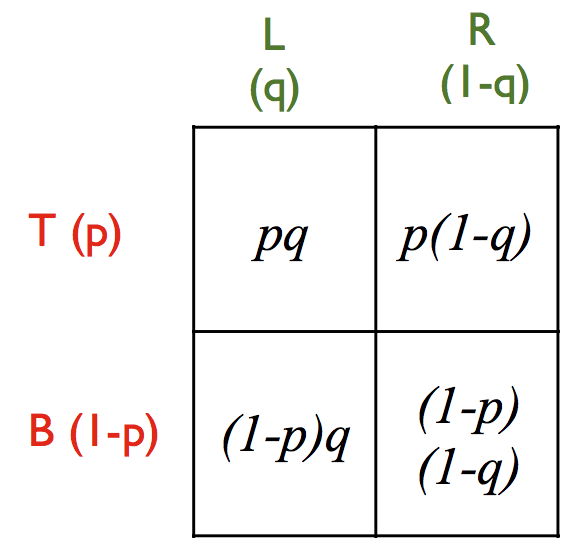
\includegraphics[scale=0.35]{figures/proba-2x2.png}
  \caption{Probabilities of a 2x2 game's matrix}
  \label{fig:proba-2x2}
\end{figure}

Thus, we have to compute the expected value of each case which means the player 1’s expected payoff for the pure strategy $Hawk(p)$ and $Dove(1-p)$, same for player 2 i.e $Hawk(q)$ and $Dove(1-q)$.

Therefore, for player 1 we obtain those equations \footnote{$U_{i}^{j}$ means the player $i$’s expected payoff for the
pure strategy $j$} : 

\begin{flalign}
 U_{1}^{H} &= q \cdot (\frac{V-D}{2}) + (1-q) \cdot V  \\
 U_{1}^{D} &= (1-q) \cdot (\frac{V}{2} - T) 
\end{flalign}

To find the value of probability $q$, we equalize the two equations to isolate $q$ : 
\begin{flalign}
 q \cdot (\frac{V-D}{2}) + (1-q) \cdot V &= (1-q) \cdot (\frac{V}{2} - T)  \\
 \frac{qV}{2} - \frac{qD}{2} + V - pV &= \frac{V}{2} - T - \frac{qV}{2} + qT \nonumber \\
 - \frac{qD}{2} &= - \frac{V}{2} - T + pT \nonumber \\ 
 \frac{qD}{2} + pT &= \frac{V}{2} + T \nonumber \\ 
 q \cdot (\frac{D}{2} + T) &= \frac{V}{2} + T \nonumber \\
 q  &= \frac{\frac{V}{2} +  T}{\frac{D}{2} + T} \nonumber \\  
 \Aboxed{q &= \frac{V+2T}{D+2T}}
\end{flalign}

By symmetry, we can deduct the equations for player 2 :  
\begin{flalign}
 U_{2}^{H} &= p \cdot (\frac{V-D}{2}) + (1-p) \cdot V  \\
 U_{2}^{D} &= (1-p) \cdot (\frac{V}{2} - T) 
\end{flalign}

therefore, the value of $p$ will be the same as $q$ too : 
\begin{flalign}
p &= \frac{V+2T}{D+2T}
\end{flalign}

which means that : 
\begin{flalign}
p = q = \frac{V+2T}{D+2T} \in [0,1] 
\end{flalign}

Therefore, for player one \textcolor{blue}{(two)}, when :
\begin{itemize}
\item $q \textcolor{blue}{(p)} > \frac{V+2T}{D+2T}$, the best response set is {$Hawk$} or $p \textcolor{blue}{(q)}=1$
\item $q \textcolor{blue}{(p)} = \frac{V+2T}{D+2T}$, the best response set is the set of all $p \textcolor{blue}{(q)}$ values in [0,1]
\item $q \textcolor{blue}{(p)} < \frac{V+2T}{D+2T}$, the best response set is {$Dove$} or $p \textcolor{blue}{(q)} =0 $
\end{itemize}

\subsection{Question 2 - Mixed strategy drawing}

\subsubsection*{Statement}

\textit{Under which conditions does displaying become more beneficial than escalating? Draw the set of all mixed strategies.} 

\subsubsection*{Graph of all mixed strategies}

Based on the calculations of probabilities $p$ and $q$ in the \autoref{sec:mixedStrat}, the graph of all mixed strategies for the Hawk-Dove game is presented in the \autoref{fig:HD-MixedStrat-Graph}. The green lines are the set of player 1's best mixed strategies while the red ones are the set of player 2's best mixed strategies. The blue circles are the mixed strategies Nash equilibria of the game. Thus, we have three possible Nash equilibria that are defined by the sets $\{(1,0);(1,0)\}, \{(0,1),(0,1)\}$ and $  \{(\frac{V+2T}{D+2T},\frac{V+2T}{D+2T}),(\frac{V+2T}{D+2T},\frac{V+2T}{D+2T})\}$.  

\begin{figure}[h]
  \centering
  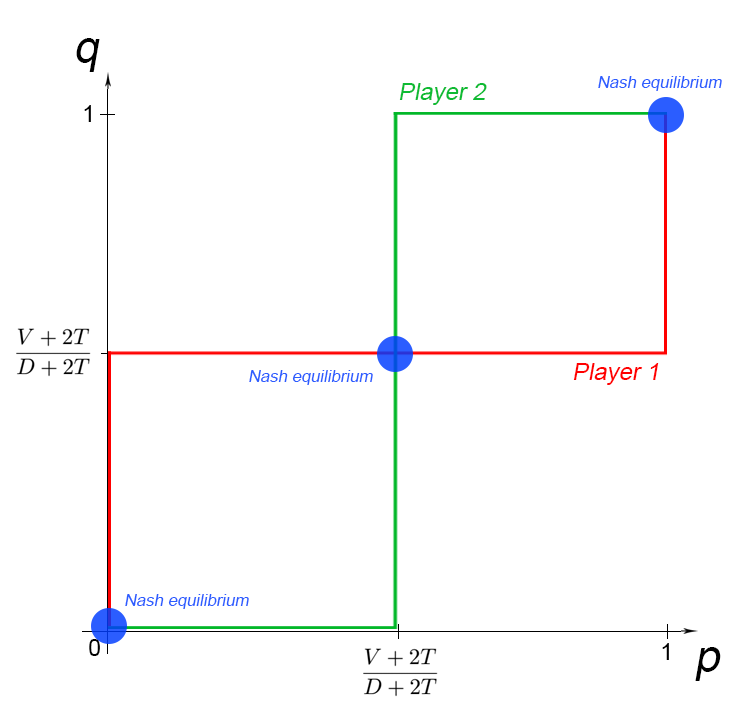
\includegraphics[scale=0.35]{figures/HD-MixedStrat-Graph.png}
  \caption{Mixed strategies graph of the Hawk-Dove game}
  \label{fig:HD-MixedStrat-Graph}
\end{figure}

\textbf{Remark} Note that $\frac{V+2T}{D+2T}$ has to be a value between 0 and 1 otherwise it wouldn't be a valid probability. Therefore, to respect this condition, necessarily $V \le D $. \\

To conclude, as calculated in the \autoref{sec:mixedStrat} and represented in the \autoref{fig:HD-MixedStrat-Graph}, if a player $i$ plays $Hawk$ with a probability $ >  \frac{V+2T}{D+2T}$ then the opponent player would play $Hawk$ because the expected value for playing $Hawk$ is higher than the expected value of playing $Dove$. Similarly, playing $Dove$ is then an optimal choice when the player $i$ chooses $Hawk$ with a probability $ < \frac{V+2T}{D+2T}$.

\newpage
\section{Which social dilemma ?}

\subsubsection*{Statement}

\textit{Player A knows he’s	confronted with	one	of three social	dilemma’s; a prisoner’s	
dilemma, a snowdrift game or stag-hunt game	(see above). In	each game he needs to decide	whether	to cooperate (C) or	defect (D),	yet	he is not sure in which	he actually	is.		He’s sure that each	game is	equally	likely.	The	other player, player B, knows in which	game he’s playing. Determine the pure Nash equilibria using	the	Bayesian game analysis	discussed in the course.} 

\subsubsection*{Data (payoff matrix) of each game}

The payoff matrix of each game is given in the statement and is taken again in the \autoref{fig:matrix-ex2}.  

\begin{figure}[h]
  \centering
  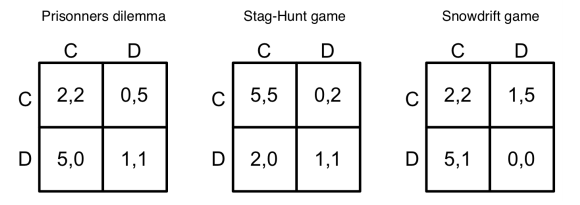
\includegraphics[scale=0.6]{figures/matrix-ex2.png}
  \caption{Payoff matrices of the prisonner's dilemma, stag-hunt and snowdrift game}
  \label{fig:matrix-ex2}
\end{figure}

\subsubsection*{Resolution}
The problem presented here is a \textit{Bayesian} game problem where a player A doesn't know which game will he play while the second player B knows it. For all cases, the player A has the choice between cooperating (C) or defecting (D). To find the Nash equilibria in such a problem, the first thing to do is to enumerate all the possibles combinations of player A's choice in each game. Let's define the set of all player $i$'s action's $\mathcal{A}_{i}$. In that case, $\mathcal{A}_{A}$ will then take those values : $\mathcal{A}_{A} = \{(C,C,C), (C,C,D), (C,D,C), (D,C,C), (C,D,D), (D,C,D), (D,D,C), (D,D,D)\}$. Concerning $\mathcal{A}_{B}$, player B has only two choices because he knows in which game he's playing, so it's simple as $\mathcal{A}_{B} = \{C,D\}$.\\

We know have all the possible actions for both player, the next step is calculating the payoff values for each combinations between an action of player A and player B. To do that, we represent $\mathcal{A}_{A}$ in the columns of the matrix and $\mathcal{A}_{B}$ in the lines of the matrix. Moreover, we know that each game is equally likely which means that every game has a probability of $\frac{1}{3}$ to be played by player A. \autoref{table:payoffMatrix-bayesian} is presenting the payoff matrix of player A for the current approached Bayesian problem. Note that the payoff values are multiplied by 3 to avoid fractions to make the matrix more clear. \\

\begin{center}
\begin{tabular}{|c|c|c|c|c|c|c|c|c|}
  \hline
  			   & CCC & CCD & CDC & DCC & CDD & DCD & DDC & DDD \\
  \hline
  C & 9 & 8 & 4 & 7 & 3 & 6 & 2 & 1 \\
  \hline
  D & 12 & 7 & 11 & 8 & 6 & 3 & 7 & 2 \\
  \hline
\end{tabular}
\captionof{table}{Payoff matrix of player A for the Bayesian game problem}
\label{table:payoffMatrix-bayesian}
\end{center}

Let's now evaluate the best responses for player A (thanks to the matrix just shown above) and for player B. To find a Nash equilibrium, the best responses of both players should match. Best responses are illustrated in \autoref{fig:BR-Bayesian} as well as the matched ones which mean the pure Nash equilibria of the problem. 

\begin{figure}[h]
  \centering
  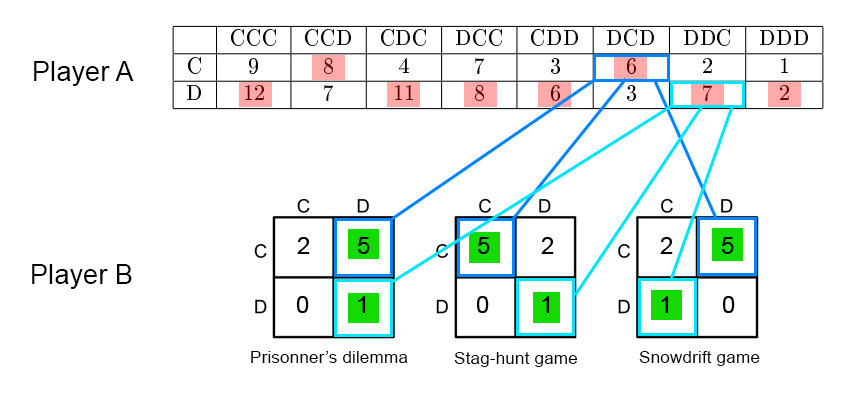
\includegraphics[scale=0.35]{figures/BR-Bayesian.png}
  \caption{Nash equilibria and best responses of the problem "Which social dilemma?" -- 
  the best responses for player A are highlighted in \colorbox{pink}{red}, the player B's ones are highlighted in \colorbox{green}{green}. The Nash equilibria are brought out in blue and cyan. }
  \label{fig:BR-Bayesian}
\end{figure}

To conclude, there exists 2 pure Nash equilibria in this problem. The first one is $(C, DCD)$ (i.e player A cooperating in the second game only while player B is cooperating) and the second one is $(D, DDC)$ (i.e player B cooperating in the last game only while player B is defecting). 

\section{Games in finite population}

\subsection*{Reminder of notations}
First, let's recap all the notations which will be used further. Denote by 
\begin{itemize}
\item $Z$, the size of the population
\item $m$, the number of rounds of the prisoner's dilemma 
\item $p_{ij}$, the \textit{fermi} function which $i$ is an individual and $j$ a population
\item $\beta$, the intensity of selection
\item $\{C,D,TFT,RANDOM\}$, respectively "always plays C", "always plays D", "play C first and then chose whichever choice the second player chose last time", "play random whether C or D each time" the 4 possibles strategies
\end{itemize}

The payoff matrix of a 2-person prisoner's dilemma is illustrated below in \autoref{fig:payoff-EX3} 

\begin{figure}[h]
  \centering
  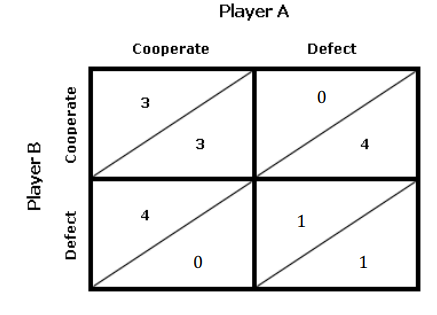
\includegraphics[scale=0.5]{figures/payoff-EX3.png}
  \caption{Payoff matrix of a 2-person prisoner's dilemma}
  \label{fig:payoff-EX3}
\end{figure}

\subsection{Question 1 - Expected payoff of strategies}

\subsubsection*{Statement}

\textit{Complete the notebook with the payoff table and copy in your answer	document the expected payoff of each strategy when facing	against	each other strategy. Use the provided python notebook ("2IPD.ipnb") to calculate the fixation probabilities of each strategy for $\beta = 10$ and paste the stationary distribution in your answer document.}

\subsubsection{Expected payoff of each strategy}
Here are the calculations of each strategy facing against each other strategy with $m = 10$ for a player $i$. As reminder, $U_{i}(a_{i},a_{-i})$ denotes the expected payoff value of the strategy $a_{i}$ against the strategy $a_{-i}$ for $m$ rounds while $u_{i}(a_{i},a_{-i})$ is for \textbf{one} round.  

\begin{flalign}
U_{i}(C,C) &= 3 \cdot m = 30 \\
U_{i}(C,D) &= 0 \cdot m = 0 \\
U_{i}(C,TFT) &= 3 \cdot m = 30 \\
U_{i}(C,RANDOM) &=  \left[\frac{1}{2} \cdot u_{i}(C,C) + \frac{1}{2} \cdot u_{i}(C,D) \right] \cdot m = (\frac{1}{2} \cdot 3 + \frac{1}{2} \cdot 0) \cdot 10 = 15 \\ \nonumber \\
U_{i}(D,C) &= 4 \cdot m = 40 \\
U_{i}(D,D) &= 1 \cdot m = 10 \\
U_{i}(D,TFT) &= u_{i}(D,C) + 1 \cdot (m-1) = 4 + 9 = 13 \\
U_{i}(D,RANDOM) &= \left[\frac{1}{2} \cdot u_{i}(D,C) + \frac{1}{2} \cdot u_{i}(D,D) \right] = (\frac{1}{2} \cdot 4 + \frac{1}{2} \cdot 1) \cdot 10 = 25 \\ \nonumber \\
U_{i}(TFT,C) &= 3 \cdot m = 30 \\
U_{i}(TFT,D) &= u_{i}(C,D) + 1 \cdot (m-1) = 0 + 9 = 9 \\
U_{i}(TFT,TFT) &= 3 \cdot m = 30 \\
  &\begin{aligned}
    \mathllap{U_{i}(TFT,RANDOM)} &= u_{i}(C,RANDOM) + \\
      &\qquad \left[\frac{1}{4} \cdot u_{i}(C,C) + \frac{1}{4} \cdot u_{i}(C,D) + \frac{1}{4} \cdot u_{i}(D,C) \frac{1}{4} \cdot u_{i}(D,D)\right] \cdot (m-1) \\
      &\qquad = \frac{5}{2} + \left[ 0 + \frac{3}{4} + 1 + \frac{1}{4} \right] \cdot 9 = 19.5 
  \end{aligned} \\
  U_{i}(RANDOM,C) &= \left[\frac{1}{2} \cdot u_{i}(C,C) + \frac{1}{2} \cdot u_{i}(D,C) \right] \cdot m = \left[\frac{1}{2} \cdot 3 + \frac{1}{2} \cdot 4 \right] \cdot 10 = 35 \\
U_{i}(RANDOM,D) &= \left[\frac{1}{2} \cdot u_{i}(C,D) + \frac{1}{2} \cdot u_{i}(D,D) \right] \cdot m = \left[\frac{1}{2} \cdot 0 + \frac{1}{2} \cdot 1 \right] \cdot 10 = 5 \\
&\begin{aligned}
    \mathllap{U_{i}(RANDOM,TFT)} &= \left[\frac{1}{2} \cdot u_{i}(C,C) + \frac{1}{2} \cdot u_{i}(D,C) \right] + \\
      &\qquad \left[\frac{1}{4} \cdot u_{i}(C,C) + \frac{1}{4} \cdot u_{i}(C,D) + \frac{1}{4} \cdot u_{i}(D,C) \frac{1}{4} \cdot u_{i}(D,D)\right] \cdot (m-1) \\
      &\qquad = \frac{7}{2} + \left[ 0 + \frac{3}{4} + 1 + \frac{1}{4} \right] \cdot 9 = 21.5 
  \end{aligned}
\end{flalign}

\begin{flalign}
    &\begin{aligned}
    \mathllap{U_{i}(RANDOM,RANDOM)} &= \left[\frac{1}{4} \cdot u_{i}(C,C) + \frac{1}{4} \cdot u_{i}(C,D) + \frac{1}{4} \cdot u_{i}(D,C) \frac{1}{4} \cdot u_{i}(D,D)\right] \cdot m   \\
      &\qquad = \left[ 0 + \frac{3}{4} + 1 + \frac{1}{4} \right] \cdot 10 = 20 
  \end{aligned}
\end{flalign}

To summerize and to make it more clear, \autoref{table:payoff-recap-EX3)} recaps all the expected payoff values for each strategy against every other strategy for $m=10$. 

\begin{center}
\begin{tabular}{|c|c|c|c|c|}
  \hline
  	\backslashbox[0pt][l]{Strat 1}{Strat 2}   & C & D & TFT & RANDOM \\
  \hline
  C & 30 & 0 & 30 & 15  \\
  \hline
  D & 40 & 10 & 13 & 25 \\
  \hline
  TFT & 30 & 9 & 30 & 19.5 \\
  \hline
  RANDOM & 35 & 5 & 21.5 & 20 \\
  \hline
\end{tabular}
\captionof{table}{Expected payoff values of 2-players prisoner's dilemma when $m=10$}
\label{table:payoff-recap-EX3)}
\end{center}

\subsubsection{Fixation probabilities}

The fixation probabilities are given in the matrix below. Respectively from left to right : $C, D, TFT$ and $RANDOM$. 

$$
\begin{bmatrix} 
 2.65746147e-10  & 9.99999973e-01 &  2.68402668e-08 &  2.65744154e-10 \\
\end{bmatrix}
$$

\subsubsection{Stationary distribution}

The stationary distribution when $\beta = 10$ is presented in the \autoref{fig:stationary-beta10}

\begin{figure}[h]
  \centering
  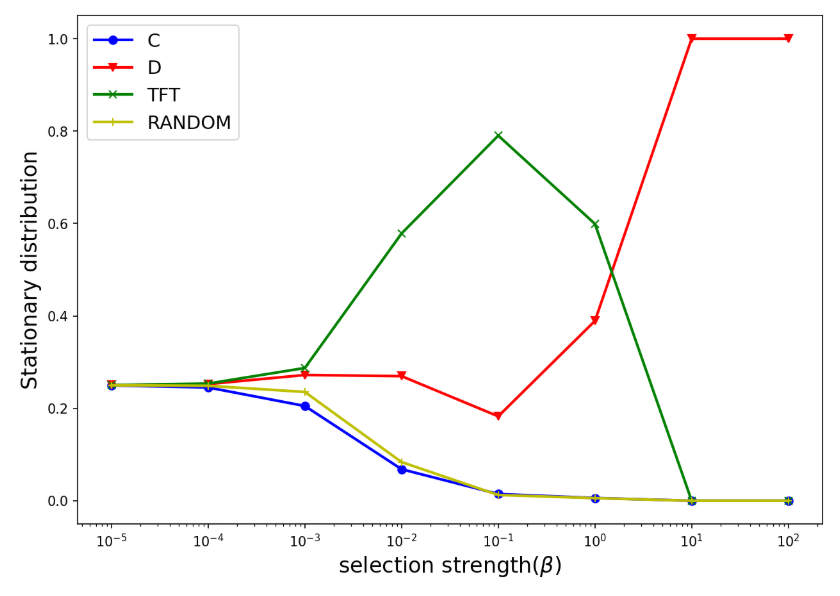
\includegraphics[scale=0.46]{figures/stationary-beta10.png}
  \caption{stationary distribution when $\beta = 10$ and $m=10$}
  \label{fig:stationary-beta10}
\end{figure}

\subsection{Question 2 - Stationary distribution for different $\beta$}

\subsubsection*{Statement}

\textit{Draw the stationary	distribution for these 4 strategies	when the mutation rate $\mu \rightarrow 0$ for different values of $\beta$.	 Paste the graph generated by the provided	python notebook in your	answer document}

\subsubsection{Result}
The mutation rate $\mu$ is denoted by the variable $drift$ in the Python notebook. When setting it at \textbf{$\beta = 0.01$} (which means $\mu \rightarrow 0$), the result of the stationary distribution for different values of $\beta$ are given below : \\

\textbf{$\beta = 10$ :} 
$$
\begin{bmatrix} 
 2.65746147e-10  & 9.99999973e-01 &  2.68402668e-08 &  2.65744154e-10 \\
\end{bmatrix}
$$

\textbf{$\beta = 5$ :} 
$$
\begin{bmatrix} 
 7.10392023e-06 &  9.99268310e-01  & 7.17495943e-04  & 7.09002624e-06 \\
\end{bmatrix}
$$

\textbf{$\beta = 1$ :} 
$$
\begin{bmatrix} 
0.00594699 & 0.38929365 & 0.5991636 &  0.00559576 \\
\end{bmatrix}
$$

What we can see from that results is that more the value of $\beta$ is small, more the stationary distribution of the strategies are high. It grows quite exponentially. 

\subsubsection{Graph}

Concerning the graph of the stationary distribution, whatever the value of $\beta$ it doesn't change anything. Therefore, the graph for every $\beta$ is given by the \autoref{fig:stationary-beta10}.


\subsection{Question 3 - Best strategy}

\subsubsection*{Statement}

\textit{Which strategy is more successful ?}

\subsubsection{Best strategy}

The best strategy is "Always play D". In the graph presented in \autoref{fig:stationary-beta10}, we can see that more the selection strength $\beta$ is high, more the strategy $D$ is increasing which shows that more	important the payoff is	in the selection process more $D$ is benefit. 

\subsection{Question 4 - $m=1$}

\subsubsection*{Statement}

\textit{What happens if $m=1$ ?}

\subsubsection{New expected payoffs}

Of course, modifying $m$ impacts the values of the expected payoff. Here are presented  these values when $m=1$. Obviously, it will also impacts the fixation probabilities values and the stationary distribution. It will be shown in the \autoref{sec:fixprob-m1} and \autoref{sec:statio-m1}. 

\begin{center}
\begin{tabular}{|c|c|c|c|c|}
  \hline
  	\backslashbox[0pt][l]{Strat 1}{Strat 2} & C & D & TFT & RANDOM \\
  \hline
  C & 3 & 0 & 3 & 1.5  \\
  \hline
  D & 4 & 1 & 4 & 2.5 \\
  \hline
  TFT & 3 & 0 & 3 & 1.5 \\
  \hline
  RANDOM & 2.5 & 0.5 & 2.5 & 2 \\
  \hline
\end{tabular}
\captionof{table}{Expected payoff values of 2-players prisoner's dilemma when $m=1$}
\label{table:payoff-recap-EX3-m1)}
\end{center}

\subsubsection{Fixation probabilities} \label{sec:fixprob-m1}

The fixation probabilities where $m=1$ are given in the matrix below. Respectively from left to right : $C, D, TFT$ and $RANDOM$. 

$$
\begin{bmatrix} 
 3.04072135e-17   1.00000000e+00   1.04488881e-17   2.61829550e-27 \\
\end{bmatrix}
$$

\subsubsection{Stationary distribution} \label{sec:statio-m1}

The stationary distribution when $\beta = 10$ and $m=1$ is presented in the \autoref{fig:stationary-beta1}

\begin{figure}[h]
  \centering
  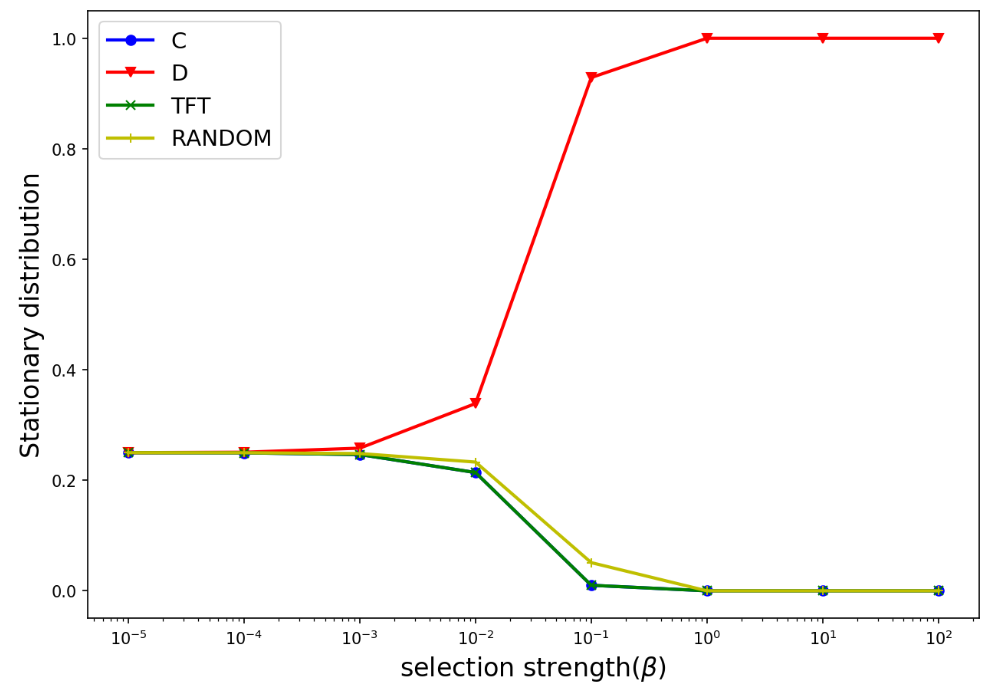
\includegraphics[scale=0.4]{figures/stationary-beta1.png}
  \caption{stationary distribution when $\beta = 10$ and $m=1$}
  \label{fig:stationary-beta1}
\end{figure}

\end{document}